\section{Zielsetzung}
\label{sec:Zielsetzung}

In diesem Versuch soll die Beugung von Licht sowohl am Einzel- als auch am Doppelspalt untersucht werden.

\section{Theorie}
\subsection{Fresnelsche und Fraunhofersche Beugung} \label{sec:FFB}
Beugung, die Ablenkung einer Welle an einem Hindernis, ist ein typisches Wellenphänomen.
Es tritt auf, wenn die Wellenlänge $\lambda$ des Lichts und die Abmessungen des Körpers, auf den dieses trifft, in der selben Größenordnung liegen. Dies lässt sich mit dem
Huygensschen Prinzip erklären, welches besagt, dass jeder Punkt einer Welle als Ursprung einer kugelförmigen Elementarwelle angesehen werden kann und die Superposition dieser
die zu betrachtende Welle ergibt. \newline
Trifft Licht auf einen Spalt, kann  dabei zwischen zwei Arten von Beugung unterschieden werden, der Fresnel- und Fraunhofer-Beugung.
Wie in Abbildung \ref{fig:beu} zu sehen ist, beschreibt die Fraunhofer-Beugung den Fall, dass Licht aus dem unendlichen auf den Spalt trifft, während
bei der Fresnel-Beugung Lichtquelle und Spalt nah beieinander liegen.  \newline
Aufgrund des geringen Abstandes treten divergente Strahlenbündel auf, sodass im Punkt $P$
Strahlen zusammentreffen, die unter verschiedenen Winkeln gebeugt werden. Dies ist bei der Fraunhofer-Beugung nicht der Fall, da dort die Strahlen aus unendlicher Entfernung nahezu parallel auf den
Spalt treffen.
\begin{figure}[H]
  \centering
  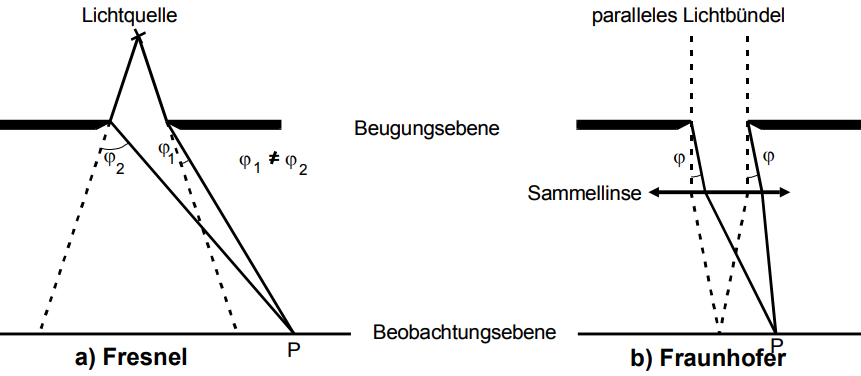
\includegraphics[width=\linewidth-30pt,height=\textheight-30pt,keepaspectratio]{Text/Bilder/Beugung.PNG}
  \caption{Schematische Darstellung der Fresnelschen und Fraunhoferschen Beugung an einem Spalt. Die gestrichelten Linien deuten den
Strahlenverlauf bei der geometrischen Optik an. \cite[31]{sample}}
  \label{fig:beu}
\end{figure}
Im Experiment kann das parallel einfallende Licht durch einen Laser realisiert werden.
Die Intensität des Lichts hinter dem Spalt in Abhängigkeit des Abstands wird dabei Beugungsfigur genannt.
Im folgendem wird ausschließlich von der Fraunhofer-Beugung ausgegangen.
\subsection{Lichtbeugung am Einzel- und Doppelspalt}
Nach den Überlegungen aus Kapitel \ref{sec:FFB} wird Licht, das auf einen Spalt trifft, gebeugt, wenn die Wellenlänge $\lambda$ des Lichts und die Spaltbreite $b$ dieselbe Größenordnung aufweisen.
Ist dabei die Breite $b$ des Spalts klein gegenüber seiner Länge, findet nur in einer Dimension Beugung statt. \newline
Einzelnde Lichtwellen laufen daraufhin am Punkt $P$ zusammen.
Sind die Lichtwellen dabei kohärent zueinander, kommt es zur Interferenz. Damit Lichtwellen kohärent zueinander sind, muss die Phasenverschiebung von aufeinander treffenden Wellen zeitlich konstant sein.
%Da die Lichtwellen in diesem Experiemt von einem Laser emitiert werden und dieser über große Kohärenzlänge verfügt, lässt sich am Punkt $p$ Interferenz beobachten.
Um die Amplitude des Lichts im Punkt $P$ zu berechnen muss daher über alle  Strahlbündel, die von sämtlichen Punkten in der Spaltöffnung in Richtung $\Psi$ emittiert werden, summiert werden.
Dazu muss zunächst die Phasendifferenz einzelner Wellen betrachtet werden.
\begin{figure}[H]
  \centering
  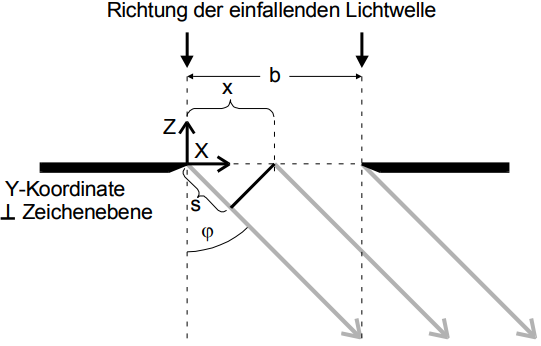
\includegraphics[width=\linewidth-30pt,height=\textheight-30pt,keepaspectratio]{Text/Bilder/Phasenbeziehung.PNG}
  \caption{Beugung am Doppelspalt \cite[34]{sample}.}
  \label{fig:phase}
\end{figure}
Aus Abbildung \ref{fig:phase} geht hervor, dass für die Phasendifferenz $\delta$ der Zusammenhang
\begin{equation}
  \delta = \frac{2 \pi s}{\lambda} = \frac{2\pi x \sin \phi}{\lambda}
\end{equation}
\begin{center}
 \small {($\lambda \: \hat{=} \:\text{Wellenlänge}$)}
\end{center}
gilt.
Unter der Annahme, dass die aus $z$-Richtung am Spalt eintreffende Welle die Form
\begin{equation}
  A(z,t) = A_0\exp \left(i\left(\omega t-\frac{2\pi z}{\lambda}\right)\right)
\end{equation}
\begin{center}
 \small {($\omega \: \hat{=} \:\text{Frequenz}$)}
\end{center}
besitzt, kann für die Amplitude $B$ in Richtung $\phi$ mit
\begin{equation}
    B(z,t,\phi) = A_0 \int_0^b\exp\left(i\left(\omega t-\frac{2\pi z}{\lambda}+\delta\right)\right)\symup{d}x\text{.}
\end{equation}
 und
 \begin{equation}
   \eta(x) = \frac{\pi x \sin \phi}{\lambda}
 \end{equation}
der Zusammenhang
\begin{equation}
  B_1(\phi) = A_0b\frac{\sin{\!\left(\eta(b)\right)}}{\eta(b)}\text{.}
\end{equation}
hergeleitet werden.
Da die Amplitude des Lichts aufgrund der hohen Frequenz nur schwer messbar ist, muss stattdessen die Intensität $I$ gemessen werden.
Es gilt der Zusammenhang
\begin{equation}
I_1(\phi)\propto B^2_1(\phi) \propto \frac{\sin^2{\!\left(\eta(b)\right)}}{\eta^2(b)}\text{.} \label{eq:I1}
\end{equation}
Die Berechnung der Intensität eines Doppelspalts verläuft analog und es ergibt sich der Zusammenhang
\begin{equation}
I_2(\phi) \propto \cos^2{\!\left(\eta(s)\right)} I_1(\phi) \propto \cos^2{\!\left(\eta(s)\right)}\frac{\sin^2{\!\left(\eta(b)\right)}}{\eta^2(b)}\text{.}\label{eq:I2}
\end{equation}
Eine schmematische Skizze des Doppelspalts befindet sich dabei in Abbildung \ref{fig:phase2}.
\begin{figure}[H]
  \centering
  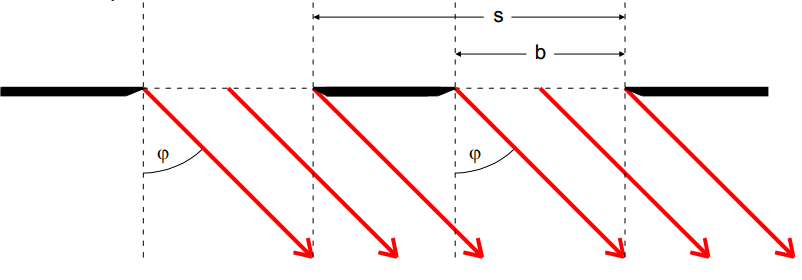
\includegraphics[width=\linewidth-30pt,height=\textheight-30pt,keepaspectratio]{Text/Bilder/Phasenbeziehung2.PNG}
  \caption{Beugung am Doppelspalt \cite[34]{sample}.}
  \label{fig:phase2}
\end{figure}
